\documentclass{standalone}
\usepackage{tikz}
\usepackage{ctex,siunitx}
\setCJKmainfont{Noto Serif CJK SC}
\usepackage{tkz-euclide}
\usepackage{amsmath}
\usetikzlibrary{patterns, calc}
\usetikzlibrary {decorations.pathmorphing, decorations.pathreplacing, decorations.shapes,}
\begin{document}
\small
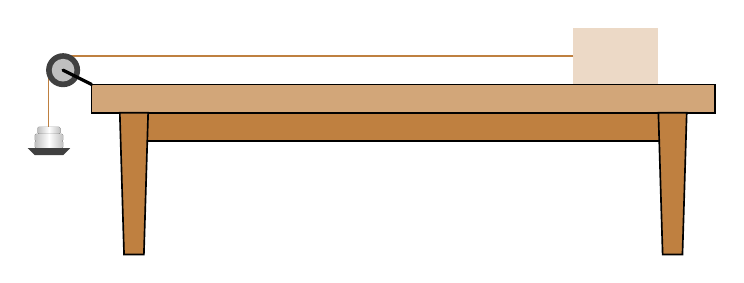
\begin{tikzpicture}[>=stealth,scale=1.8]
  \fill [brown!30](1.2,2.0)rectangle(1.8,2.4);
  \draw [semithick,fill=brown!70](-2.2,1.8)rectangle(2.2,2);
  \draw [semithick,fill=brown](-1.9,1.8)rectangle(1.9,1.6);
  \draw [semithick,fill=brown](-2.0,1.8)--(-1.97,0.8)--(-1.83,0.8)--(-1.8,1.8)--cycle;
  \draw [semithick,fill=brown](2.0,1.8)--(1.97,0.8)--(1.83,0.8)--(1.8,1.8)--cycle;
  \draw [brown] (1.2,2.2)--(-2.4,2.2);
  \draw [brown] (-2.5,2.1)--(-2.5,1.7);
  \fill [darkgray] (-2.4,2.1)circle(0.12);
  \fill [lightgray] (-2.4,2.1)circle(0.08);
  \draw [very thick,line cap=round](-2.4,2.1)--(-2.2,2);
  \fill [left color=lightgray,right color=lightgray, middle color=white,rounded corners=0.15mm](-2.42,1.7)rectangle(-2.58,1.65);
  \fill [left color=lightgray,right color=lightgray, middle color=white,rounded corners=0.15mm](-2.4,1.65)rectangle(-2.6,1.6);
  \fill [left color=lightgray,right color=lightgray, middle color=white,rounded corners=0.15mm](-2.4,1.6)rectangle(-2.6,1.55);
  \fill [darkgray](-2.35,1.55)--(-2.65,1.55)--(-2.6,1.5)--(-2.4,1.5);
\end{tikzpicture}
\end{document}